\documentclass[12pt,letterpaper]{article}
\usepackage[utf8]{inputenc}
\usepackage[spanish]{babel}
\usepackage{graphicx}
\usepackage[left=2cm,right=2cm,top=2cm,bottom=2cm]{geometry}
\usepackage{graphicx} % figuras
\usepackage{subfigure} % subfiguras
\usepackage{float} % para usar [H]
\usepackage{amsmath}
\usepackage{txfonts}
\usepackage{stackrel} 
\usepackage{multirow}
\usepackage{enumerate} % enumerados
\renewcommand{\labelitemi}{$-$}
\renewcommand{\labelitemii}{$\cdot$}
\author{Fanny Clemente}
\title{Caratula}
\begin{document}

% Fancy Header and Footer
\usepackage{fancyhdr}
\pagestyle{fancy}
\cfoot{}
\rfoot{\thepage}
%

\usepackage[hidelinks]{hyperref} % CREA HYPERVINCULOS EN INDICE

\author{Fanny Clemente}
\title{Caratula}

\begin{titlepage}
\begin{center}
\large{UNERSIDAD PRIVADA DE TACNA}\\
\vspace*{-0.025in}
\begin{figure}[htb]
\begin{center}

\includegraphics[width=8cm]{./Figuras/logo}
\end{center}
\end{figure}
\vspace*{0.15in}
INGENIERIA DE SISTEMAS  \\

\vspace*{0.5in}
\begin{large}
TITULO:\\
\end{large}

\vspace*{0.1in}
\begin{Large}
\textbf{TRABAJO ENCARGADO} \\
\end{Large}

\vspace*{0.3in}
\begin{Large}
\textbf{CURSO:} \\
\end{Large}

\vspace*{0.1in}
\begin{large}
BASE DE DATOS II\\
\end{large}

\vspace*{0.3in}
\begin{Large}
\textbf{DOCENTE(ING):} \\
\end{Large}

\vspace*{0.1in}
\begin{large}
 Patrick Cuadros Quiroga\\
\end{large}

\vspace*{0.2in}
\vspace*{0.1in}
\begin{large}
Integrantes: \\
\begin{flushleft}
Acevedo Vásquez, Leonardo Fernando 	(2014047512) \\
Andía Bernedo, Josei Jomar 			(2014049093) \\
Condori Velarde, Sonia          	(2014049546) \\
Clemente Cruz, Fanny Luz    		(2014049550) \\
Flores Colque, Gisela           	(2014049547) \\
Llatasi Cohaila, Cristian Omar		(2014037546) \\
Morales Anquise, Tommy Edwards 		(2015050480) \\
Ticona Arcaya, Sergio Alexis		(2014049171) \\
Tapia Ticona, Lupe Carolina			(2014049548) \\
\end{flushleft}
\end{large}
\end{center}

\end{titlepage}




 \tableofcontents
 \newpage



\section{Seccion 4} 
\subsection{Oracle SQL Developer Data Modeler}
\subsubsection{Ejercicio 0: Instalacion de Oracle SQL Developer Data Modeler.}
		descripcion general  \\
En esta practica, se instalaran Orcale SQL Developer Data Modeler. Siga las instrucciones en funcion de si dispone de un sistema operativo Windows, Mac o Linux. \\
\\
Supuestos\\
Debe haber descargado los archivos de instalacion de Orcale Technology Network. Puedo descargar archivos desde el enlace proporcionado:
http://www.oracle.com/technetwork/developer-tools/datamodeler/downloads/index.html\\
\\
Tareas\\
Para realizar las instaalcion en una plataforma windows de 32 bits o 64 bits:
\begin{enumerate}[1.]
    \item Asegúrese de que tiene instalado un JRE, de lo contrario, descargue el JRE del sitio web de Oracle Technology Network .  \\
    Nota: El enlace para descargar el JRE es: http://www.oracle.com/technetwork/java/javase/downloads/index.html
    
   \item Descargue el archivo zip de Data Modeler.
   
   \item Extraiga el archivo zip en cualquier carpeta.
   
   \item Acceda al interior de esa carpeta.
   
    \item Amplíe la carpeta datamodeler.
    
    \item Haga doble clic en datamodeler.exe para 32 bits y haga doble clic en datamodeler64.exe para 64 bits.
   
		\end{enumerate} 
		
	
Para realizar la instalacion en una plataforma Linux::
\begin{enumerate}[1.]
    \item Asegurese de que tiene instalado un JRE, de lo contrario, descargue el JRE de Oracle Technology .  \\
    Nota: El enlace para descargar el JRE es: http://www.oracle.com/technetwork/java/javase/downloads/index.html
    
   \item Descargue el archivo <datamodeler...noarch.rpm>.
   
   \item Para extraer el archivo rpm, ejecute el siguiente comando:\\
   rpm -Uhv <datamodeler...noarch.rpm>
   
   \item Suponiendo que el archivo rpm se ha extraído en la carpeta /opt/datamodeler, defina los privilegios:\\
   chmod -R 777 /opt/datamodeler
   
    \item Ejecute Data Modeler, conectándose como usuario configurado.
    
    \item Defina la variable de entorno de zona horaria ejecutando el siguiente comando:\\
    export TMZ="GMT"
   
		\end{enumerate}
		
		
		
		Para realizar la instalacion en una plataforma Mac:
\begin{enumerate}[1.]
    \item Asegurese de que tiene instalado un JRE.  \\
    Tenga en cuenta que el enlace para descargar el JRE es: http://developer.apple.com/java/download/
    
   \item Descargue el archivo zip (archivo de almacenamiento)
   
   \item Extraiga el archivo en cualquier carpeta.
   
   \item Haga clic dos veces en el archivo OracleDataModeler.app.

		\end{enumerate}
Tareas\\
Para su comodidad, aquí se muestra un resumen de cómo funciona la base de datos académica (sistema de gestión de escuela):
\begin{enumerate}[1.]
\item Una escuela/universidad tiene diferentes departamentos que ofrecen cursos a los alumnos en una determinada sesión académica.
\item Cada uno de estos cursos lo imparte un profesor.
\item Los alumnos pueden inscribirse en diferentes cursos en una sesión académica.
\item Además de los detalles de registro, la universidad/escuela debe mantener también la información principal sobre el alumno.
\item El departamento mantiene los detalles de asistencia del alumno, que determinarán si un alumno puede optar a los exámenes de esa sesión académica o no.
\item Para cada sesión académica, se realizan exámenes y los resultados se comparten con el alumno en un período de tiempo estipulado.
\item El departamento también mantiene un registro del tiempo de conexión y desconexión del profesorado para sus necesidades de generación de informes.
\end{enumerate}
Con la información proporcionada anteriormente, utilice Oracle SQL Developer Data Modeler para identificar y crear:
\begin{itemize}
    \item Las entidades del sistema de gestión de escuela.
    \item Los atributos para cada una de las entidades identificadas.
    \item La relación entre las entidades.    
\end{itemize}
\begin{center}
    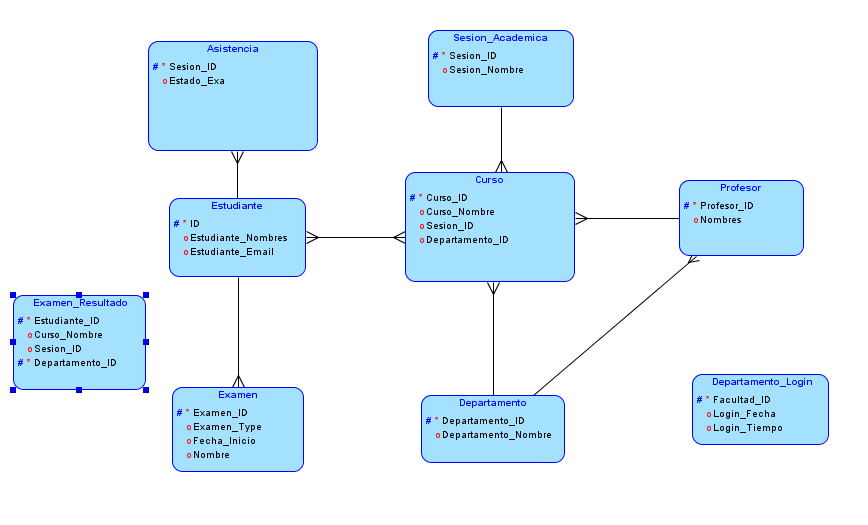
\includegraphics[width=16cm]{./IMAGENES/bd222222222222222222222.png} 
\end{center}




 \newpage
\subsection{Convert a Logical Model to a Relational Model}
 \newpage
\subsubsection{Ejercicio 1: Ingenieria Directa de un Modelo Logico en un Modelo Relacional.} 
descripcion general  \\
En esta práctica realizara ingeniería directa del modelo logico de la base de datos academica en un modelo relacional con Oracle SQL Developer Data Modeler. \\

Tareas\\
Para realizar la ingeniería directa del modelo logico de la base de datos academica a un modelo relacional, realice lo siguiente:

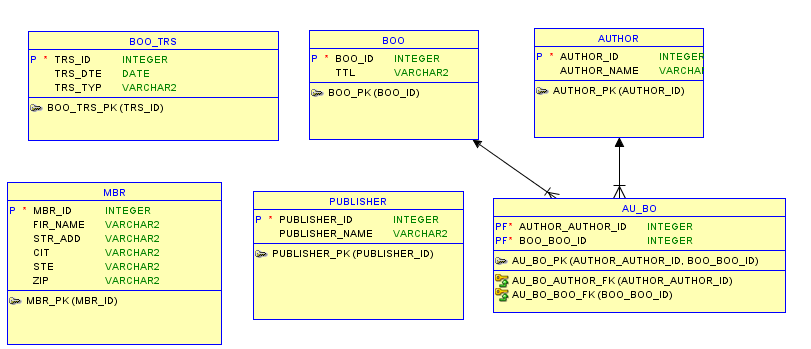
\includegraphics[width=15cm]{./soniaImagen/diagrama1.png} 

\begin{enumerate}[1.]
    \item  Abra el modelo logico en Oracle SQL Developer Data Modeler.
    
    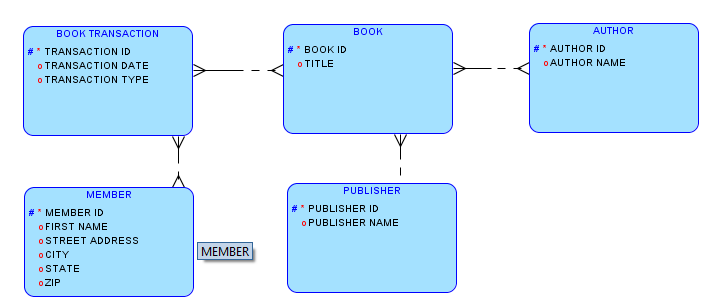
\includegraphics[width=15cm]{./soniaImagen/diagrama2.png} 
     
    \item SHaga clic en el icono Engineer to Relational Model.
    
   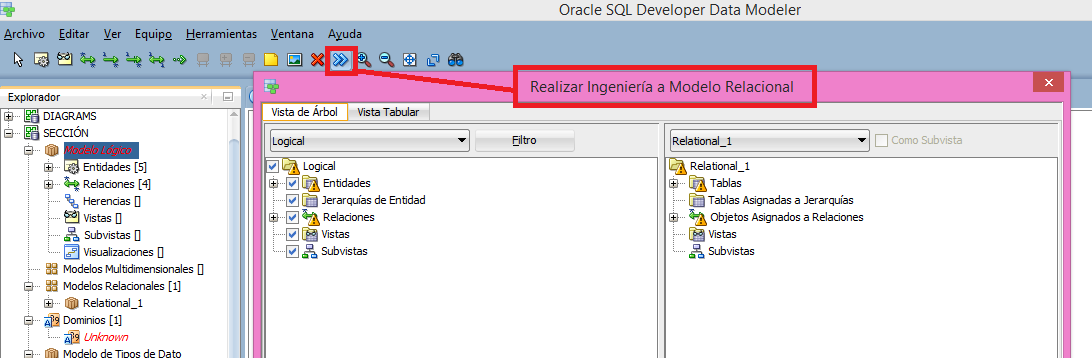
\includegraphics[width=15cm]{./soniaImagen/diagrama3.png} 
    
    \item Acepte todos los valores por defecto y haga clic en Engineer.
    
      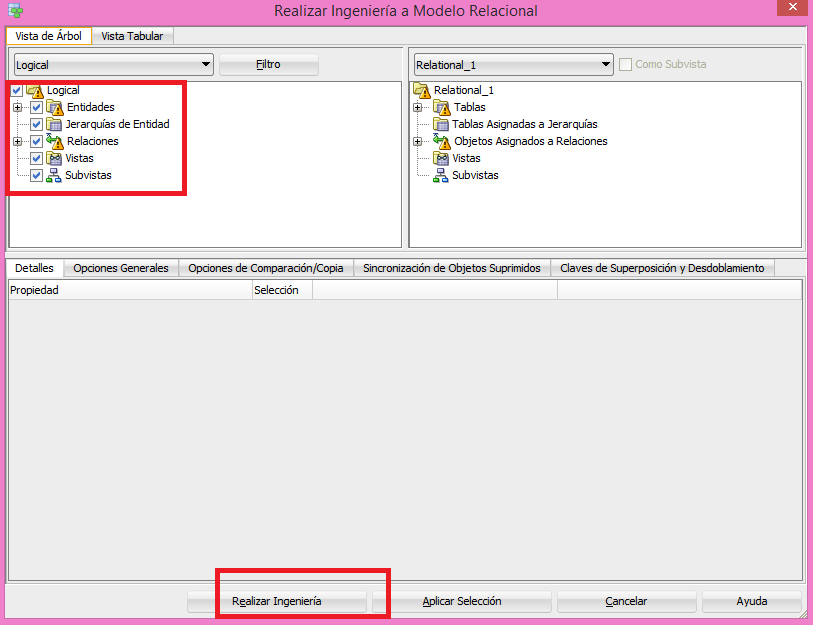
\includegraphics[width=15cm]{./soniaImagen/diagrama4.png}  
    
     \item Expanda el nodo Relational Models en el explorador de objetos para ver los objetos creados.
     
          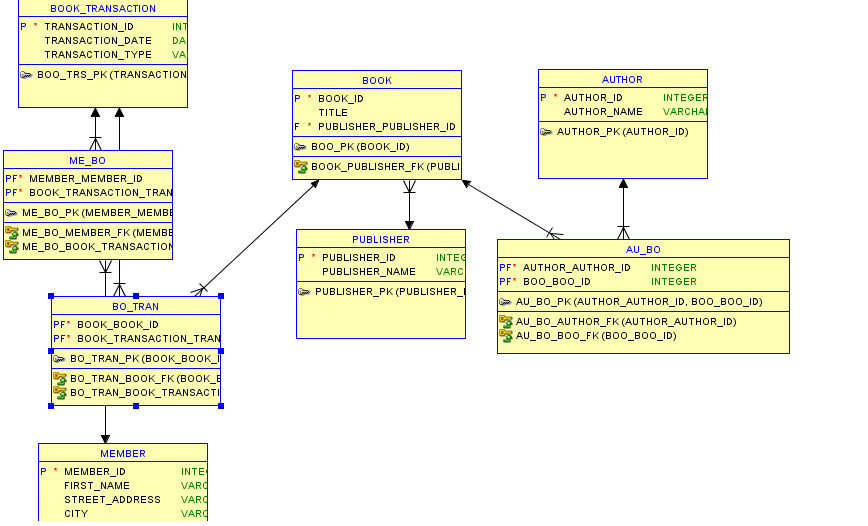
\includegraphics[width=15cm]{./soniaImagen/diagrama5.png}  
          
		\end{enumerate}



\subsubsection{Ejercicio 2: Ingenieria Inversa de un Modelo Relacional en un Modelo Logico.} 
descripcion general  \\
En esta practica, agregará una nueva columna al modelo relacional de ingenieria en la practica 2-1 y, a continuacion, realizara ingenieria inversa del modelo relacional en el modelo logico. \\
Supuestos\\
Ha terminado la practica 2-1.\\
\\
Tareas\\
Agregue una columna a una de las tablas del modelo relacional. En la siguiente captura de pantalla, la columna EMAILADDR se agrega a la tabla ADPARENTINFORMATION.


 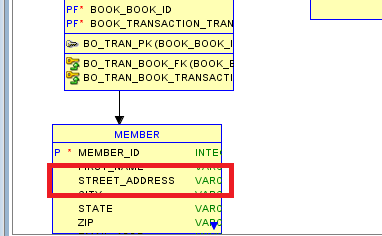
\includegraphics[width=15cm]{./soniaImagen/diagrama6.png}  

Ahora, para realizar la ingenieria inversa del modelo relacional de la base de datos academica a un modelo logico con los cambios, realice lo siguiente: \\
\begin{enumerate}[1.]
    \item  Haga clic en el icono Engineer to Logical Model. 
    
       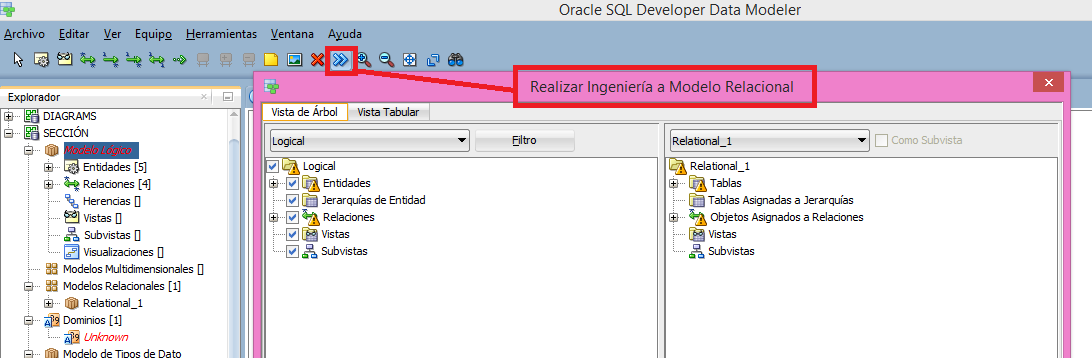
\includegraphics[width=15cm]{./soniaImagen/diagrama3.png} 
     
    \item Acepte todos los valores por defecto y haga clic en Engineer.
    
       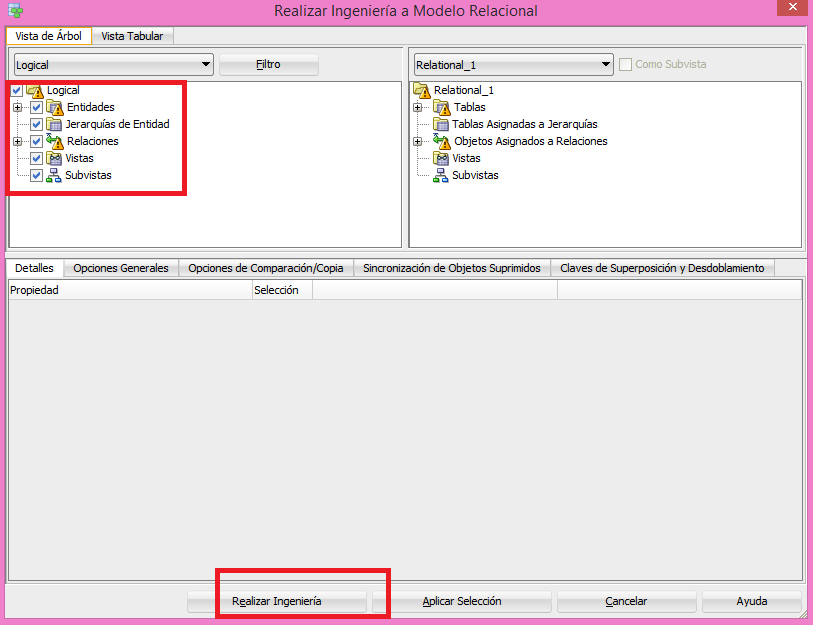
\includegraphics[width=15cm]{./soniaImagen/diagrama4.png}  
    
    \item Acepte todos los valores por defecto y haga clic en Engineer.
    
      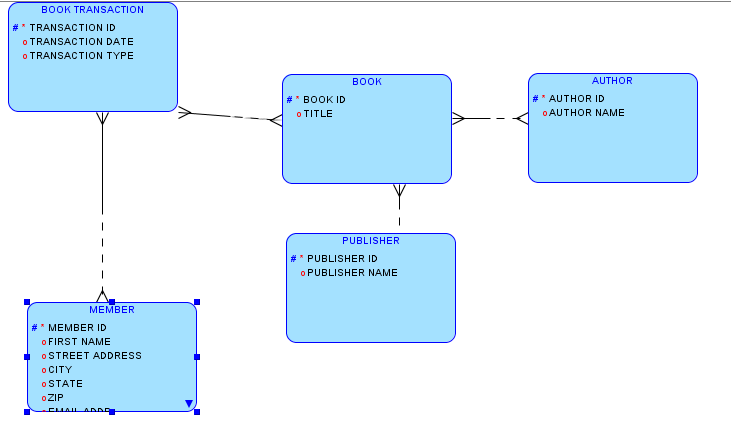
\includegraphics[width=15cm]{./soniaImagen/diagrama7.png} 
    
		\end{enumerate}






 \newpage
\section{seccion 5} 
\subsection{Mapping Entities and Atributes}
\subsubsection{Ejercicio 1: Creacion de un Glosario a Partir del Modelo Logico.} 
descripcion general  \\
En esta practica, creara un glosario a partir del modelo logico de la base de datos academica. \\

Tareas\\
\begin{enumerate}[1.]
    \item  Abra el modelo logico de la base de datos academica 
     
    \item Haga clic con el boton derecho en el nodo Logical Model en el explorador y seleccione "Create Glossary from Logical Model"
    
    \item Especifique el nombre del glosario, una breve descripcion y tantos tipos de clasificacion como sean aplicables a las entradas del glosario.
    
    \item Guarde el glosario.
    
		\end{enumerate}












 \newpage
\subsection{Mapping Primary and Foreign Keys}
\subsubsection{Ejercicio 1: Observacion de la Asignacion de indentificadores unicos y su relacion en el modelo relacional.} 
Descripcion general \\
en esta practica observara la asignacion de los identificadores unicos y su relacion en el mdelo relaiconal de la base de datos academica. \\
TAREAS\\
los identiicadors unucos que se han asignado como claves primarias\\
 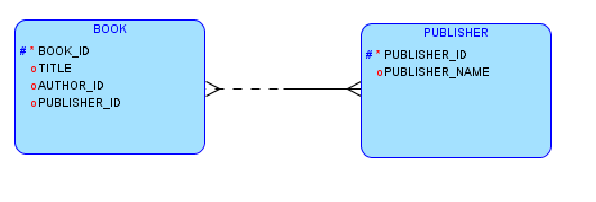
\includegraphics[width=15cm]{./giselaImagen/imagen1.png} 
		\\ Modelo Relacional:
		
 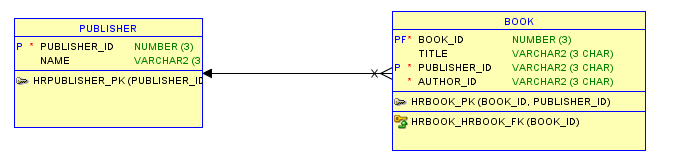
\includegraphics[width=15cm]{./giselaImagen/imagen2.png} 
		\\ Modelo Relacional

los idetificaadores unicos que se han asignado como claves unicas\\
 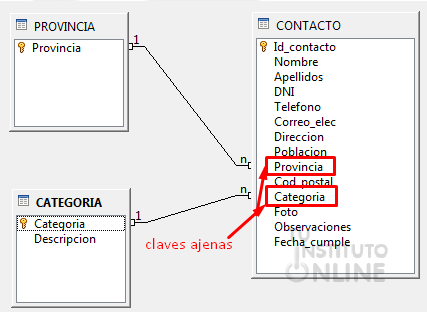
\includegraphics[width=15cm]{./giselaImagen/imagen3.png} 
		\\ Modelo Relacional
Las relaciones que se han asignado como claves ajenas. \\
 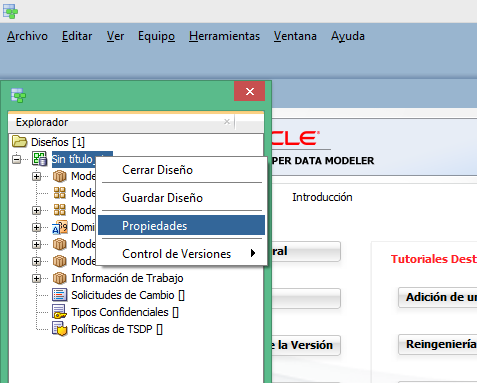
\includegraphics[width=15cm]{./giselaImagen/imagen4.png} 
		\\ Modelo Relacional
		\subsubsection{Ejercicio 2: Definicion de la plantilla.}
		descripcion general  \\
En esta practica , definira plantilla patrones de nombre para claves, indices y restriciones mediante el uso de combinaciones de variables predefinidas. \\

Tareas
\begin{enumerate}[1.]
    \item Puede definir un aplantilla para claves, indice y restriciones en la tabla o entidad utilizando combnaiones de variabes predefinidas. para defiir los patrones de nombre, realice los siguientes pasos .  \\
haga clic en el boton derecho en el diseno de la base de datos academico en el explorador de objetos y selecciones Properties. Ampie Settinga Naming Standard y selecciones Templates. \\
 Defina las variables predefinidas de la siguiente forma. 
    
		\end{enumerate}
		\subsubsection{Ejercicio 3: Aplicacion de plantilla de nombre al modelo relacional.}
		descripcion general  \\
Despues de definir la plantilla de nomenclatura pudede aplicarlo a una entidad/tabla o a todo el modelo logico/relacional. En esta practica, aplicara la plantillaa de nomenclatura a todo el modelo relacional \\

Tareas\\
para aplicar la pantilla a todo el modelo relacional, reaalice lo siguiente. 
\begin{enumerate}[1.]
    \item En el explorador de objetos, haga clic con el boton derecho en el modelo relacional, y a continuacion , seleccione Apply Naming Standars to Keys and Constraints en el menu emergente. Se muestra el cuadro de dialogo Apply Naming Standards. 
    
     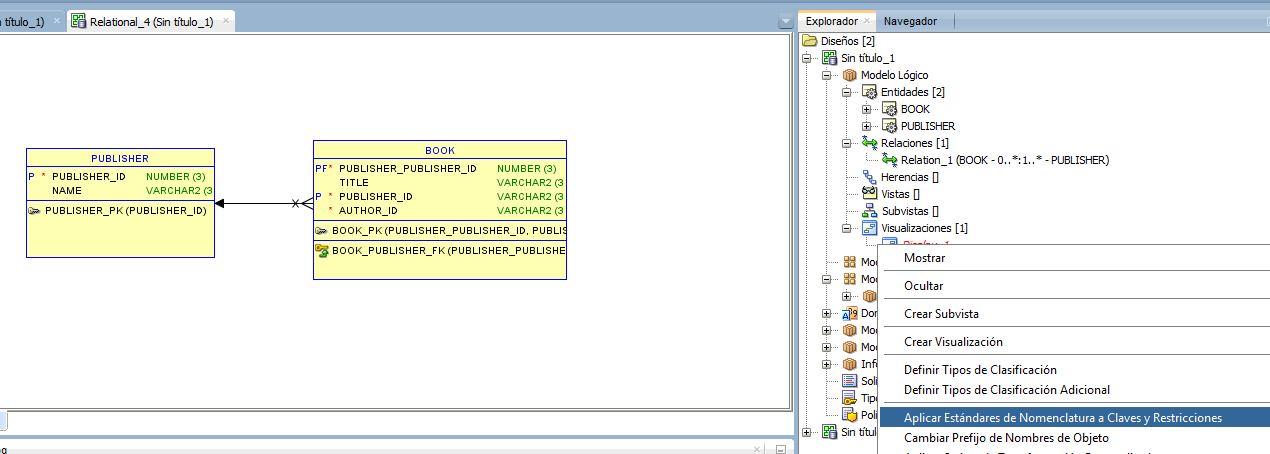
\includegraphics[width=15cm]{./giselaImagen/imagen6.png} 
     
    \item Selecione los tipos de objetyo a los que se desea aplicar las plantillasy , a continuacion, haga clic en OK. 
    
    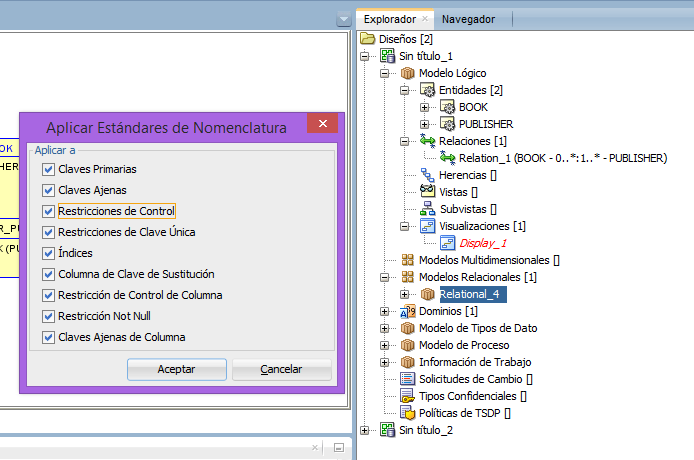
\includegraphics[width=15cm]{./giselaImagen/imagen7.png} 
    
    \item observe que se aplica la plantilla.  
		\end{enumerate}
		
		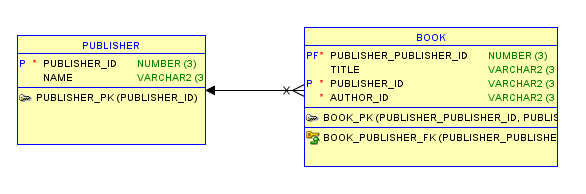
\includegraphics[width=15cm]{./giselaImagen/imagen8.png} 
		
		\subsubsection{Ejercicio 4: Aplicacion de un Prefijo de nombre de objeto a los objetos del Modelo Relacional.}
		descripcion general  \\
Den esta practica, aplicara un prefijo de nombre de objeto al modelo relacional de la base de datos academica. \\

Tareas\\
para aplicar el prefijo de nombre de objeto al modelo relacional de la base de datos academica, realice los siguientes pasos.  
\begin{enumerate}[1.]
    \item Haga clic con el boton derecho en el modelo relacionaly, a continuacion, seleccione Change Object Names Prefix. 
    
    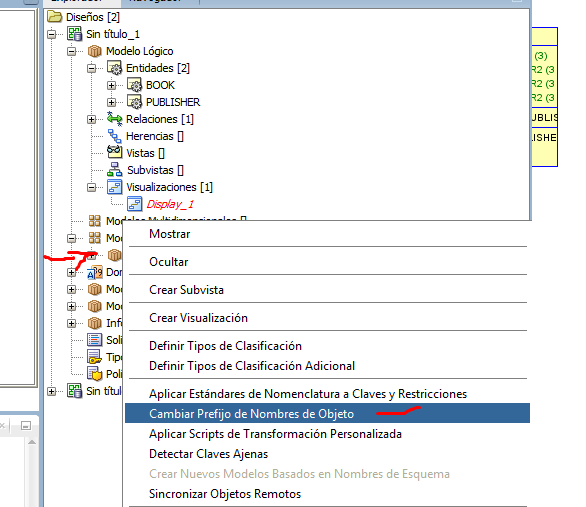
\includegraphics[width=15cm]{./giselaImagen/imagen9.png} 
    
    \item Esecifique un nuevo prefijo (en este cado AD), haga clic en Add new prefix, seleccione los objetos a los que se desea aplicarselo y, a continuacion, haga clic en aplicar. 
    
    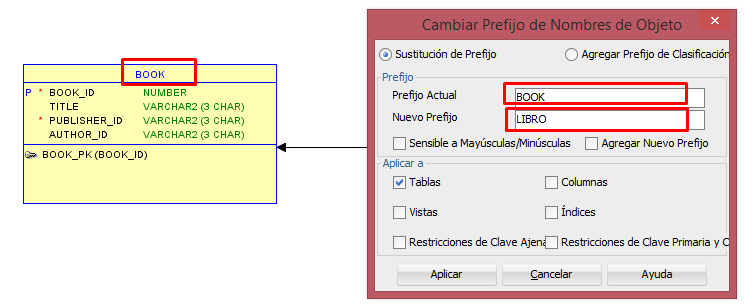
\includegraphics[width=15cm]{./giselaImagen/imagen10.png} 
    
    \item Se mustra el cuadro de dialogo de mensaje que indica cuantos nombres han cambiado.  
    
    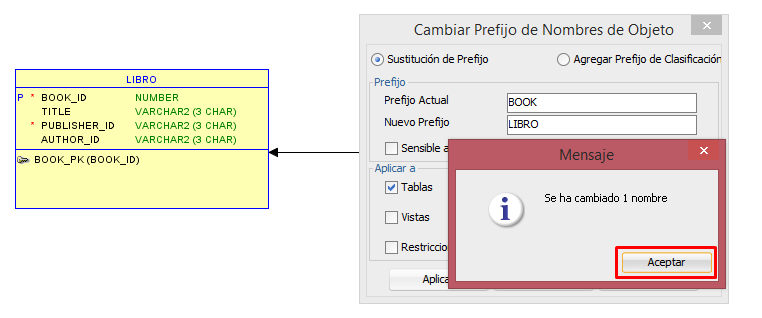
\includegraphics[width=15cm]{./giselaImagen/imagen11.png} 
    
    \item Tenga en cuenta que los nombres de las tablas tiene n ahora enl prefijo.  
		\end{enumerate}
		
		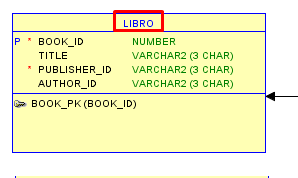
\includegraphics[width=15cm]{./giselaImagen/imagen12.png} 













 \newpage
 
\section{seccion 6 } 
\subsection{Introduction to Oracle Aplication Express}

\subsubsection{Ejercicio 1: Introduccion a Oracle Application Express} 
descripcion general  \\
En esta practica, vera un documento que le guiara por las distintas funciones de Oracle Application Express. \\

Tareas\\

\begin{enumerate}[1.]
    \item  Navegue a la Seccion 0 de este curso y haga clic para acceder a la Guia del Usuario de APEX.. 
     
    \item Siga la Guia del Usuario para acceder a Oracle Application Express y conocer las funciones de
Oracle Application Express.

		\end{enumerate}









\newpage
\subsection{Structured Query Language (SQL)}

\subsubsection{Ejercicio 1: Uso de la Ayuda de Oracle Application Express} 
descripcion general  \\
En esta practica:\\
 Se conectará a Oracle Application Express\\
 Se familiarizara con las secciones Help de Oracle Application Express \\
 \\
Supuestos\\
Se le ha asignado un espacio de trabajo de Oracle Application Express y las credenciales para conectarse.\\
\\
Tareas\\
Acceda y conectese a Oracle Application Express
\\
\\
Haga clic en el icono Help y familiaricese con la siguiente seccion y temas: \\
\begin{enumerate}[1.]
    \item  Guia del Taller de SQL de Oracle Application Express. 
     
    \item Gestion de Objetos de Base de Datos con el Explorador de Objetos.
    
    \item Uso de Comandos SQL.
    
     \item Uso de Scripts SQL.
    
    
		\end{enumerate}
		




\newpage
\subsection{Data Definition Language (DDL)} 

\subsubsection{Ejercicio 1: Creacion de Tablas con Oracle Application Express} 
descripcion general  \\
En esta practica, creara las tablas para la base de datos academica. \\
 \\
Supuestos\\
A continuacion, se muestra el diagrama de relacion de entidad (ERD) para la base de datos en la que se crearan las tablas:\\


Tareas\\
\begin{enumerate}[1.]
    \item  Cree las sentencias DDL para crear las tablas de la base de datos academica mostradas anteriormente.  
     
    \item Ejecute estos comandos en Oracle Application Express.
    
		\end{enumerate} 
		
		
		
		\subsubsection{Ejercicio 2: Modificacion de Tablas} 
descripcion general  \\
En esta practica:\\
Modificara las tablas para definir las restricciones\\
Especificará un valor por defecto para una columna\\
Definirá una tabla en estado de solo lectura\\
 \\
Supuestos\\
Los nombres de tabla se basan en las tablas creadas en la practica 3-2.\\


Tareas\\
\begin{enumerate}[1.]
    \item  Modifique las tablas de la base de datos academica para definir las restricciones de clave primaria y clave ajena.  
     
    \item Modifique la tabla AD FACULTY LOGIN y especifique un valor por defecto para la columna LOGIN DATE.
    
    \item Modifique la tabla AD STUDENT para agregar una columna que contenga la direccion de correo electronico. Defina esta columna como unica..
    
    \item Defina la tabla AD PARENT INFORMATION en un estado de solo lectura.\\
    Nota: Puede escribir las sentencias ALTER TABLE y guardarlas como un script .sql que, posteriormente, se podrá copiar y ejecutar en APEX.
    
    
		\end{enumerate} 
		
	
	
	\subsubsection{Ejercicio 3: Creacion de Claves Primarias, Ajenas y unicas Compuestas} 
descripcion general  \\
En esta practica, creara una:\\
Clave primaria compuesta\\
Clave ajena compuesta\\
Clave unica compuesta\\
 \\

Tareas\\
\begin{enumerate}[1.]
    \item  Cree la tabla DEPT con la siguiente estructura:  
     
    \item Cree las tablas SUPPLIERS y PRODUCTS con la siguiente estructura:
    
    \item Cree la tabla DEPT SAMPLE con la siguiente estructura:
    
   
    
		\end{enumerate} 
		




\newpage
\subsection{Data Manipulation Language (DML)} 

		\subsubsection{Ejercicio 1: Insercion de Filas en Tablas} 
descripcion general  \\
Insertara filas en las tablas creadas para la base de datos academica\\
 \\
Supuestos\\
Las tablas se han creado para la base de datos academica (basada en la práctica 3).\\


Tareas\\
\begin{enumerate}[1.]
    \item Inserte filas en las tablas creadas para la base de datos academica.  
     
    
    
		\end{enumerate} 
		
		\subsubsection{Ejercicio 2: Actualizacion de Filas en las Tablas} 
descripcion general  \\
Actualizara los registros de la tabla de detalles de alumnos para incluir las direcciones de correo electronico de los alumnos.\\
 \\
Supuestos\\
La tabla que contiene los detalles de los alumnos es AD STUDENT DETAILS.\\
Oracle Application Express se ha iniciado en un explorador.\\


Tareas\\
\begin{enumerate}[1.]
    \item En la practica 3 se ha modificado la tabla de detalles de alumnos para incluir una columna denominada direccion de correo electronico. Utilice Oracle Application Express para comprobar qué datos se han almacenado para esa columna.  
     \item Actualice la columna de direccion de correo electronico en la tabla de detalles de alumnos.\\
    Nota: Puede escribir las sentencias UPDATE y guardarlas como un script .sql que, posteriormente, se puede cargar y ejecutar en Oracle Application Express.\\
    
		\end{enumerate}





\newpage
\subsection{Transaction Control Language (TCL)} 


\subsubsection{Ejercicio 1: Control de Transacciones} 
descripcion general  \\
En esta practica, controlara las transacciones mediante las siguientes sentencias:
COMMIT\\
ROLLBACK\\
SAVEPOINT\\
 \\
Supuestos\\
Para trabajar con las sentencias de control de transacciones, creará una tabla de prueba, AD STUDENT TEST DETAILS.\\
Se trabajara sobre la transaccion en la tabla de prueba\\


Tareas\\
\begin{enumerate}[1.]
    \item Cree una tabla de prueba con la siguiente estructura.  
     \item Modifique la tabla para agregar la columna email addr:.\\
   \item Cree un punto de grabacion denominado ALTER DONE.
     \item Realice rollback en la sentencia hasta el punto de grabacion ALTER DONE. ¿Observa los cambios?.
      \item Inserte filas en la tabla de prueba o cree un punto de grabacion denominado INSERT DONE.
      \item Actualice una fila en la tabla de prueba o cree un punto de grabacion denominado UPDATE DONE. 
      \item Suprima una fila de la tabla de prueba o cree un punto de grabacion denominado DELETE DONE
     \item  Realice rollback hasta el punto de grabacion UPDATE DONE. ¿Que cambios observa respecto a las transacciones?\\
      NOTA: Las tareas anteriores no se pueden realizar en Oracle Application Express. Utilice Oracle SQL Developer para trabajar con las tareas.
		\end{enumerate}





\newpage
\subsection{Retrieving Data using SELECT)}
\subsubsection{Ejercicio 1: Recuperacion de columnas de las tablas} 
descripcion general  \\
Seleccionar todas las columnas de una tabla\\
Seleccionar columnas especificadas de una tabla\\
\\
SUPUESTOS \\
Utilizara Oracle Aplication Express parea consultar las tablas\\
\\Tareas
\begin{enumerate}[1.]
    \item Escriba una consulta simple para ver los datos insertados en las tablas creadas para la base de datos.
    
\begin{center}
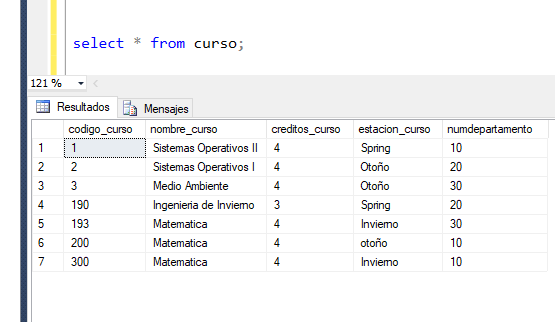
\includegraphics[width=15cm]{./IMAGENES/imagen6_1}
\end{center}

    
    
    \item Escriba una consulta para recuperar las calificaciones obtenidas por el alumno para cada examen realizado.
    
    
\begin{center}
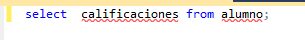
\includegraphics[width=12cm]{./IMAGENES/imagen6_2}
\end{center}

    
    \item Escriba una consulta para comprobar si un alumno puede realizar examenes en funcion de numero de dias que ha asistido a clase.
    
     
\begin{center}
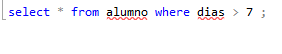
\includegraphics[width=12cm]{./IMAGENES/imagen6_3}
\end{center}


    \item Muestre los valores LOGIN DATE y LOGIN TIME de cada miembro de profesorado.
    
    
\begin{center}
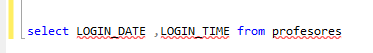
\includegraphics[width=12cm]{./IMAGENES/imagen6_4}
\end{center}

    
    
    \item Muestre el nombre del jefe del departamento de todos los departamentos.
    
     
\begin{center}
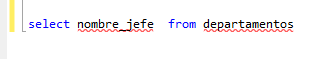
\includegraphics[width=12cm]{./IMAGENES/imagen6_5}
\end{center}



    \item Recupere el identificador de alumno y el nombre de cada alumno concatenados po el literal " : "(dos puntos). 
    

\begin{center}
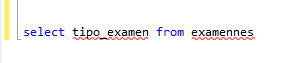
\includegraphics[width=12cm]{./IMAGENES/imagen6_7}
\end{center}


    \item Muestre todos los tipos de examen distintos de la tabla AD EXAM DETAILS.   
\end{enumerate}


\begin{center}
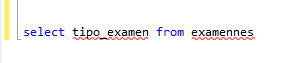
\includegraphics[width=12cm]{./IMAGENES/imagen6_7}
\end{center}

\newpage
\subsubsection{Ejercicio 2: Uso de Operadores Aritmeticas y Alias de Columna en Sentencias SELECT} 
descripcion general  \\
En esta practica, utilizara operadores aritmeticas y alias de columna en sentencias SELECT.\\
\\
Tareas \\
\begin{enumerate}[1.]
     \item El profesorado de los distintis departamentos observo que las calificaciones introducidas en AD EXAM RESULTS mostraban un aumento de 5 putos por cada entrada. ¿se puede mostrar las calificaciones restando 5 puntos a las calificaiones obtenidas por cada alumno?
     

\begin{center}
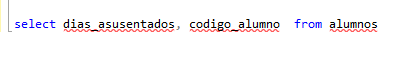
\includegraphics[width=12cm]{./IMAGENES/imagen6_2_2}
\end{center}

     
     
       
    \item Muestre el porcentaje de dias que se han ausentado los alumos y su idoneidda para relizar los examenes.
    
   
\begin{center}
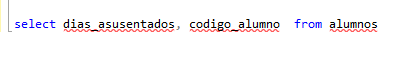
\includegraphics[width=12cm]{./IMAGENES/imagen6_2_2}
\end{center}

    
    \item Muestre los valores FIRST NAME y EMAIL ADDR como "The email address of < FIRST NAME > is <EMAIL ADDR>".
    
   
\begin{center}
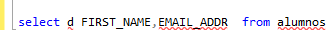
\includegraphics[width=12cm]{./IMAGENES/imagen6_2_3}
\end{center}

  
    \item Muestre el nombre y el HOD del departamento de la tabla AD DEPARTMENT.
    
   
\begin{center}
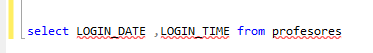
\includegraphics[width=12cm]{./IMAGENES/imagen6_4}
\end{center}

     
      
    \item Muestre los distintos DEPARTMENT ID de la tabla AD COURSE DETAILS.   
\end{enumerate}


\begin{center}
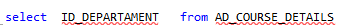
\includegraphics[width=12cm]{./IMAGENES/imagen6_2_5}
\end{center}

     










\newpage
\subsection{Restricting Data Using WHERE} 
\subsubsection{Ejercicio 1: Restriccion de Datos mediante SELECT} 
descripcion general  \\
En esta practica, limitada las filas mostradas con:\\
Claususla WHERE\\
Los operadores de comparacion\\
Condiciones logicas mediante los operadores AND , OR y NOT.\\
\\
\\Tareas
\begin{enumerate}[1.]
    \item Muestre los detalles del curso para la sesion Spring

\begin{center}
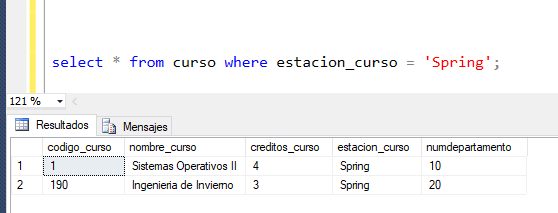
\includegraphics[width=12cm]{./IMAGENES/imagen1}
\end{center}

    
    \item Muestre los detalles de los alumnos que han conseguido una puntuacion superior a 97.
    
 
\begin{center}
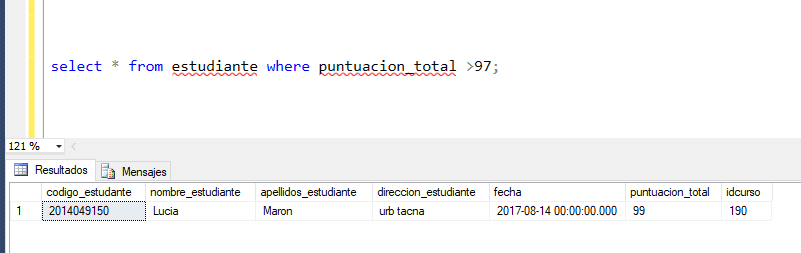
\includegraphics[width=12cm]{./IMAGENES/imagen2}
\end{center}


    \item Muestre los detalles de los alumnos que han conseguido una puntuacion entre 65 y 70.

\begin{center}
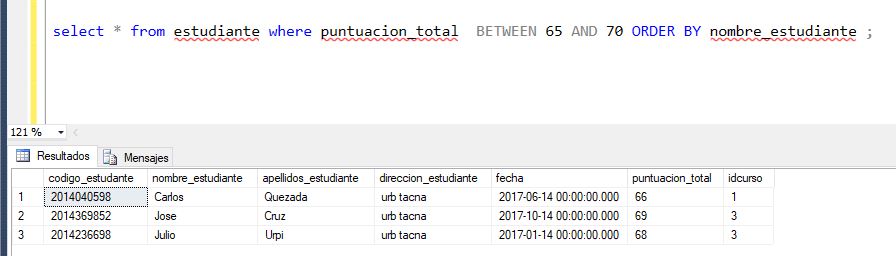
\includegraphics[width=12cm]{./IMAGENES/imagen3}
\end{center}


    
    \item Muestre a los alumnos que se registraron despues del 01-Jun-2012.
    

\begin{center}
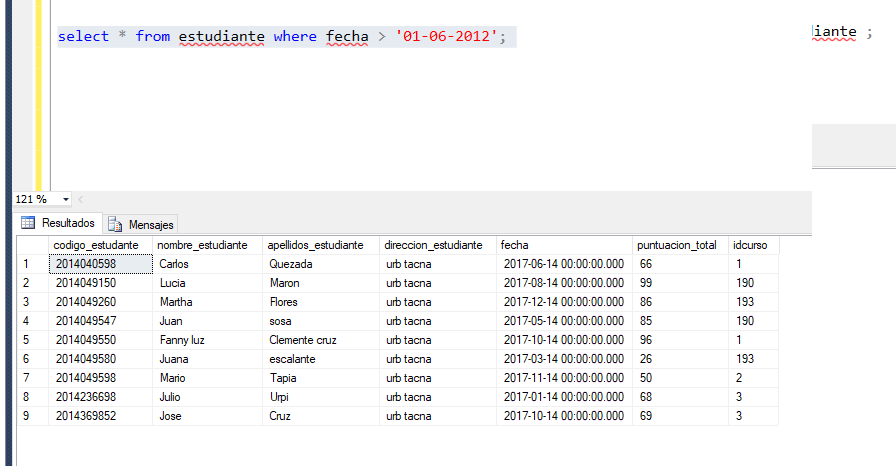
\includegraphics[width=12cm]{./IMAGENES/imagen4}
\end{center}

    \item Muestre los detalles del curso para los departamentos 10 y 30. 
    
  
\begin{center}
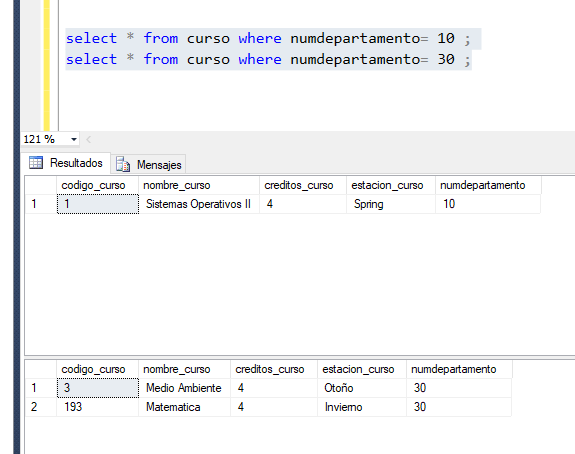
\includegraphics[width=12cm]{./IMAGENES/imagen5}
\end{center}

    \item Muestre los detalles de los alumnos cuyos nombres empiecen por la letra "J". 
  
\begin{center}
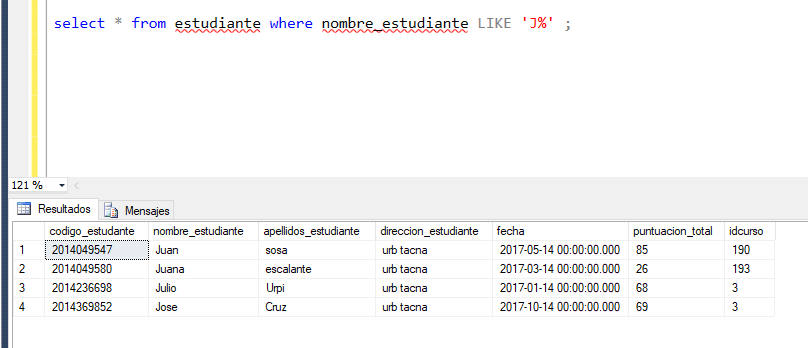
\includegraphics[width=12cm]{./IMAGENES/imagen6}
\end{center}



    \item Muestre los detalles de los alumnos que han optado por los cursos 190 o 193.

\begin{center}
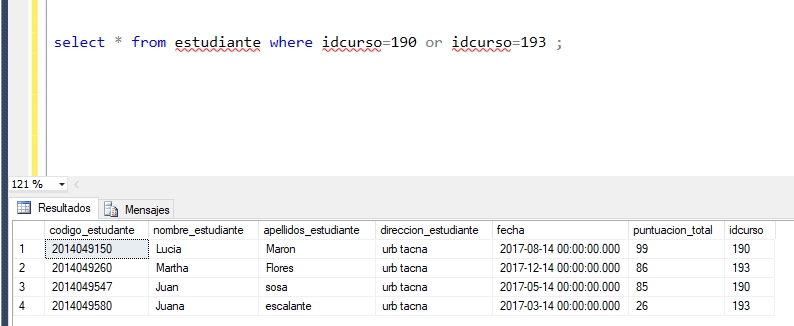
\includegraphics[width=12cm]{./IMAGENES/imagen7}
\end{center}

    \item Muestre los detalles del curso ofrecidos por el departamento 30 para la sesion de otono (identificador de sesion 200).
    

\begin{center}
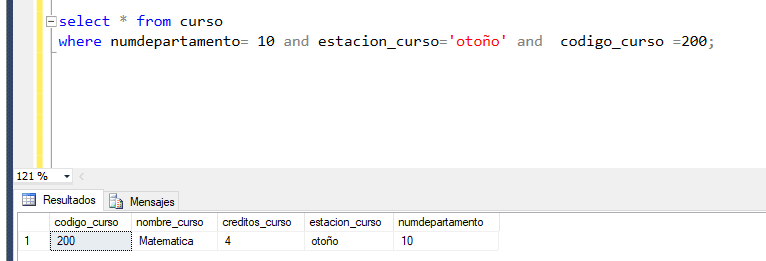
\includegraphics[width=12cm]{./IMAGENES/imagen8}
\end{center}

    
    \item  Muestre los detalles de los cursos no ofertados en la sesion de verano y otono (identificador de sesion 200 y 300).
    
 
\begin{center}
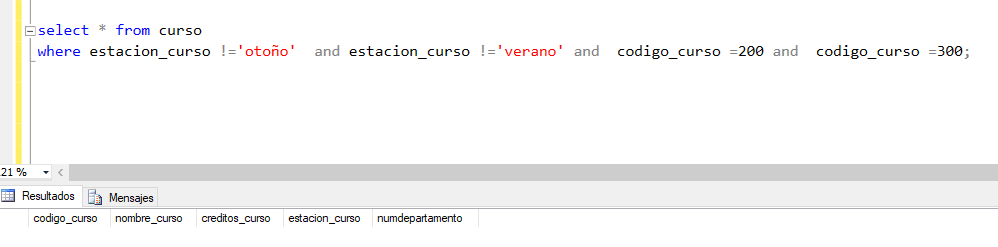
\includegraphics[width=12cm]{./IMAGENES/imagen9}
\end{center}

    \item Muestre los detalles del curso para el departamento 20.

\begin{center}
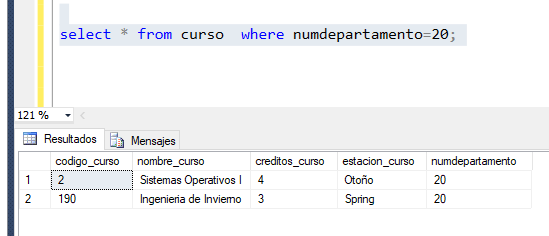
\includegraphics[width=12cm]{./IMAGENES/imagen10}
\end{center}


   
\end{enumerate}








\newpage
\subsection{Sorting Data Using ORDER BY} 

\subsubsection{Ejercicio 1: Ordenacion de Datos mediante ORDER BY} 
descripcion general  \\
En esta practica:\\
Ordenacion de filas mediante la clausula ORDER BY\\
 Ordenacion de datos y limitacion de la salida de filas mediante la clausula SQL de limitacion de filas
 \\
Supuestos\\
Para trabajar con las sentencias de control de transacciones, creará una tabla de prueba, AD STUDENT TEST DETAILS.\\
Se trabajara sobre la transaccion en la tabla de prueba\\


Tareas\\
\begin{enumerate}[1.]
    \item Muestre los registros en orden ascendente para las siguientes tablas:\\

\begin{enumerate}
	\item	Muestre los registros en orden ascendente para las siguientes tablas:\\

		a.	AD STUDENT DETAILS ordenado por STUDENT REG YEAR\\ 
		
			Select * from adStudentDetails order by studentRegYear ASC;\\	
			
		b.	AD EXAM RESULTS ordenado por STUDENT ID y COURSE ID\\ 
		
			Select * from adExamResults order by studentId , courseId\\
					
		c.	AD STUDENT ATTENDANCE ordenado por STUDENT ID\\ 

			Select * from adStudentAttendance order by studentid ASC;\\
		
		d.	AD DEPARTMENT ordenado por DEPARTMENT ID\\

			Select * from addepartment order by  departmentid  ASC;\\
 
	\item	Muestre el porcentaje de d�as que se han ausentado los alumnos y ordene los registros seg�n el porcentaje calculado.\\
	
		SELECT NoOfDaysOff * 100/(SELECT sum(NoOfDaysOff) AS porcentajeDeFaltas FROM STUDENT ATTENDANCE) 
		FROM STUDENT ATTENDANCE GROUP BY NoOfDaysOff;\\
 
	\item	Muestre los 5 alumnos con la mayor calificaci�n y, a continuaci�n, los siguientes 5 alumnos, es decir,  los clasificados del 6 		al 10.\\

		SELECT dem�sAtributos, MAX(atributoNota) from TablaAlumnos ORDER BY atributoId DESC LIMIT 5 \\
 
	\item	Utilice WITH TIES para devolver todas las filas que tienen la misma clave de ordenaci�n que la �ltima fila de la cl�usula 			de limitaci�n de filas cuando muestra 5 alumnos.\\
	
		SELECT TOP (5) WITH TIES StudentId from STUDENT ORDER BY StudentId DESC;\\
 
	\item	Muestre los detalles principales ordenados por "PARENT ID".\\
	
		SELECT * FROM TablaDetalles ORDER BY PARENT ID ASC;\\

\end{enumerate}
\end{enumerate}
\newpage
\subsection{Joining Tables Using JOIN} 

\subsubsection{Ejercicio 1: Uso de UNIONES en Consultas SQL} 
descripcion general  \\
En esta practica, debera:
Acceder a los datos de más de una tabla con uniones igualitarias y no igualitarias\\
Utilizar uniones EXTERNAS para visualizar datos que normalmente no cumplen una condicion de union\\
Generar un producto cartesiano\\
 \\

Tareas\\
\begin{enumerate}[1.]
    \item Muestre los diferentes cursos que ofertan los departamentos de la escuela\\

     \item MMuestre los cursos que se ofertan en otono.\\

    \item Muestre los detalles del curso, el departamento que ofrece los cursos y los alumnos que se han inscrito en esos cursos.
    \item Muestre los detalles del curso, el departamento que ofrece los cursos y los alumnos que se han inscrito en esos cursos del departamento 30.
    \item ¿Se ejecutara correctamente la sentencia especificada? En caso negativo, ¿que se debe cambiar?
      
    \item Escriba una consulta para mostrar los detalles de las calificaciones obtenidas por los alumnos que han optado por el curso con COURSE ID en el rango de 190 a 195.
      
    \item Recupere las filas de la tabla AD EXAM RESULTS incluso si no hay ningun registro que coincida en la tabla AD COURSE DETAILS.
      
    \item ¿Que salida se debe generar cuando se ejecuta la sentencia especificada?
		\end{enumerate}





\end{document}
